\section{Solution}
\label{sec:solution}

\subsection{Cluster Analysis Results Visualization}
\label{sec:cluster}

As was discussed before in the Section~\ref{sec:dataset_description} cluster analysis result graph is binary tree.

"A binary tree is a connected acyclic graph such that the degree of each vertex is no more than 3. A rooted binary tree is such a graph that has one of its vertices of degree no more than 2 singled out as the root. With the root thus chosen, each vertex will have a uniquely defined parent, and up to two children; however, so far there is insufficient information to distinguish a left or right child. If we drop the connectedness requirement, allowing multiple connected component in the graph, we call such a structure a forest"~\cite{BINARY_TREE} Simple binary tree showed on the Figure~\ref{fig:simple_binary_tree}

\begin{figure}[h!]
\centering
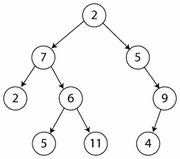
\includegraphics[scale=1.0]{pictures/simple_binary_tree.png}
\caption{A simple binary tree graph}
\label{fig:simple_binary_tree}
\end{figure}

There several visualization methods for binary trees and more specific methods for cluster result. The main method for visualizing clusters is - dendrogram. Here is sample dendrogram visualization on the Figure~\ref{fig:dendrogram_1} produced by MATLAB 7.2.

\begin{figure}[h!]
\centering
\subfloat[Dendrogram]{
    \label{fig:dendrogram_1}
    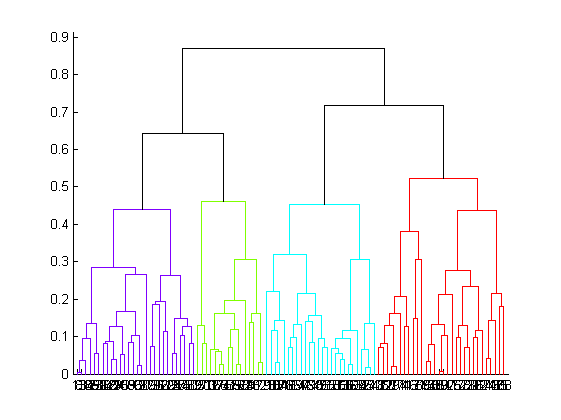
\includegraphics[scale=0.45]{pictures/dendrogram.png}
}
\subfloat[Polar Dendrogram]{
    \label{fig:polardendrogram}
    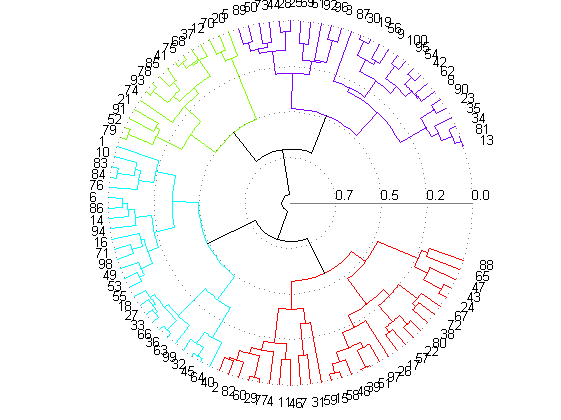
\includegraphics[scale=0.45]{pictures/polardendrogram.png}
}
\label{fig:dendrograms}
\caption{Cluster visualisations}
\end{figure}


The Figure~\ref{fig:polardendrogram} shows polar dendrogram visualization algorithm of the same cluster tree produced by MATLAB.

One of the main ideas was to use polar dendrogram algorithm for cluster visualization. The Figure~\ref{fig:JUNG_radial_layout} shows visualization of the Cluster using native JUNG radial layout algorithm. Red are nodes and white is edges, black is background. As picture shows algorithm doesn't count nature of the cluster - very deep binary tree not wide as it is common for cluster analysis results, that's why it has many edge everlappings.


\begin{figure}[h!]
\centering
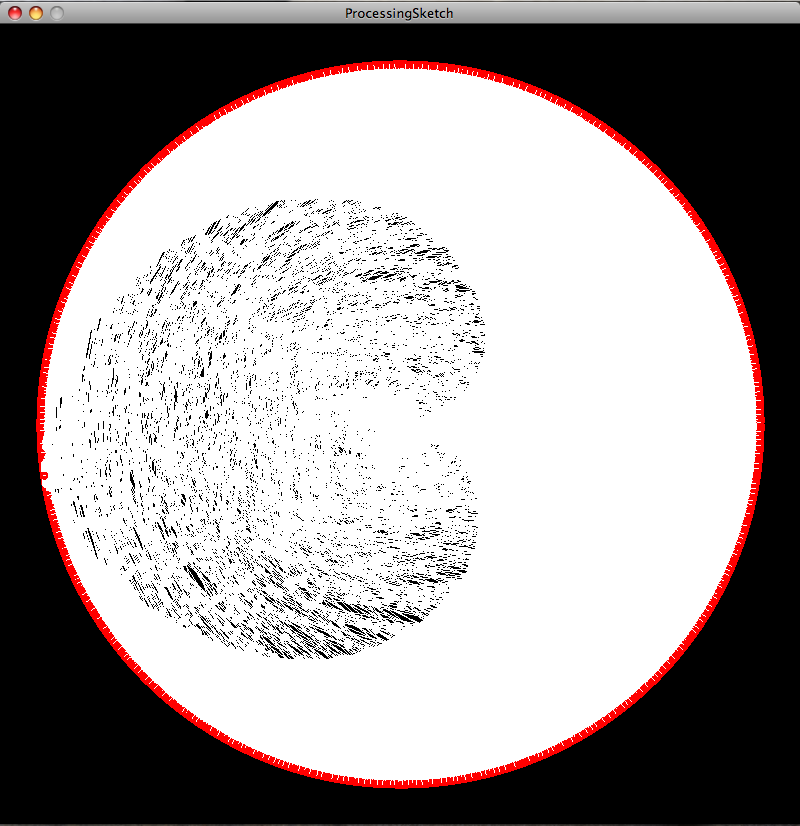
\includegraphics[scale=0.4]{pictures/using_JUNG_radial.png}
\caption{Cluster visualization using JUNG radial layout}
\label{fig:JUNG_radial_layout}
\end{figure}


Also to visualization issue it has performance issue -- without any measurement was seen for an eye that program does not allow smooth interaction. Low performance issue was in nature of the visualization in the JUNG: it uses very complex hierarchical structure with many utility classes per visualized object and the cost is big memory usage. Also JUNG uses Java 2D~\cite{JAVA_2D} which by itself is "heavyweight" because it's part of the Java AWT -- Abstract Windows Toolkit.


"The Abstract Window Toolkit (AWT) is Java's original platform-independent windowing, graphics, and user-interface widget toolkit. The AWT is now part of the Java Foundation Classes (JFC) � the standard API for providing a graphical user interface (GUI) for a Java program. When Sun Microsystems first released Java in 1995, AWT widgets provided a thin level of abstraction over the underlying native user interface. For example, creating an AWT check box would cause AWT directly to call the underlying native subroutine that created a check box."~\cite{JAVA_AWT} This technology is outdated and replaced by Swing.


"Swing is the primary Java GUI widget toolkit. It is part of Sun Microsystems' Java Foundation Classes (JFC) � an API for providing a graphical user interface (GUI) for Java programs.
Swing was developed to provide a more sophisticated set of GUI components than the earlier Abstract Window Toolkit. Swing provides a native look and feel that emulates the look and feel of several platforms, and also supports a pluggable look and feel that allows applications to have a look and feel unrelated to the underlying platform."~\cite{JAVA_SWING}


"Since early versions of Java, a portion of the Abstract Window Toolkit (AWT) has provided platform-independent APIs for user interface components. In AWT, each component is rendered and controlled by a native peer component specific to the underlying windowing system.
By contrast, Swing components are often described as lightweight because they do not require allocation of native resources in the operating system's windowing toolkit. The AWT components are referred to as heavyweight components."~\cite{JAVA_SWING} More detail comparison can be found here.~\cite{AWT_VS_SWING}


The Figure~\ref{fig:cluster_jogl_impl} shows improved JUNG radial algorithm and own visualization implementation using JOGL. JOGL will be discussed in the Section~\ref{sec:opengl}.


\begin{figure}[h!]
\centering
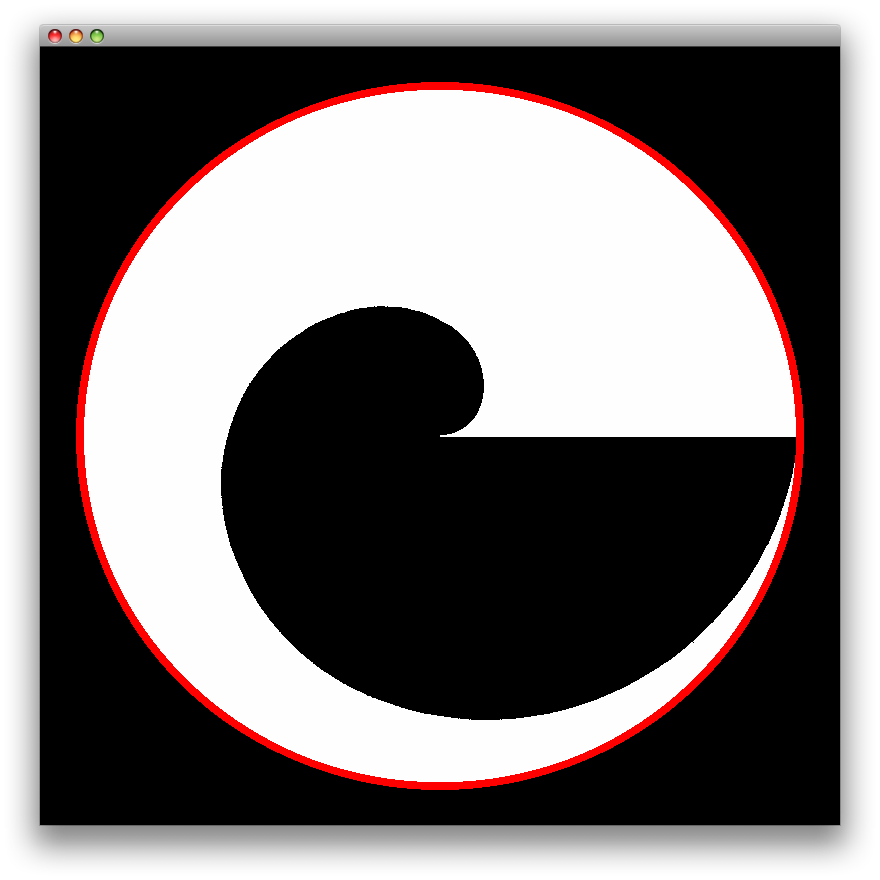
\includegraphics[scale=0.4]{pictures/cluster_jogl_impl.png}
\caption{Cluster visualization using JOGL and improved JUNG radial layout}
\label{fig:cluster_jogl_impl}
\end{figure}


The Figure~\ref{fig:cluster_jogl_impl_with_subgraph_1} and Figure~\ref{fig:cluster_jogl_impl_with_subgraph_2} shows cluster visualization and highlighted subgraph using algorithm that was discussed in the Section~\ref{sec:problem}. This pictures show the nature of the dataset. Improved version has good performance and better visualization but still has issues - there are too many elements in the scene, it is impossible to identify separate gene or trace highlighted graph genes.

\begin{figure}[h!]
\centering
\subfloat[Cluster graph and highlighted subgraph]{
    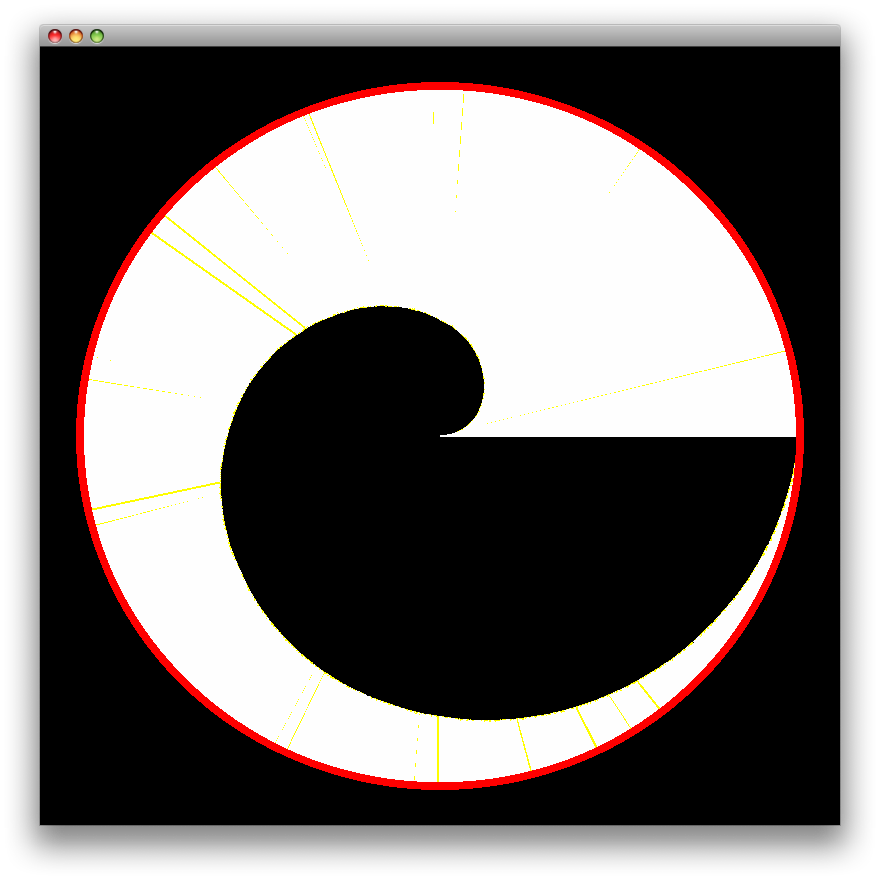
\includegraphics[scale=0.2]{pictures/cluster_jogl_impl_with_subgraph_1.png}
    \label{fig:cluster_jogl_impl_with_subgraph_1}
}
\subfloat[Cluster graph and highlighted subgraph]{
    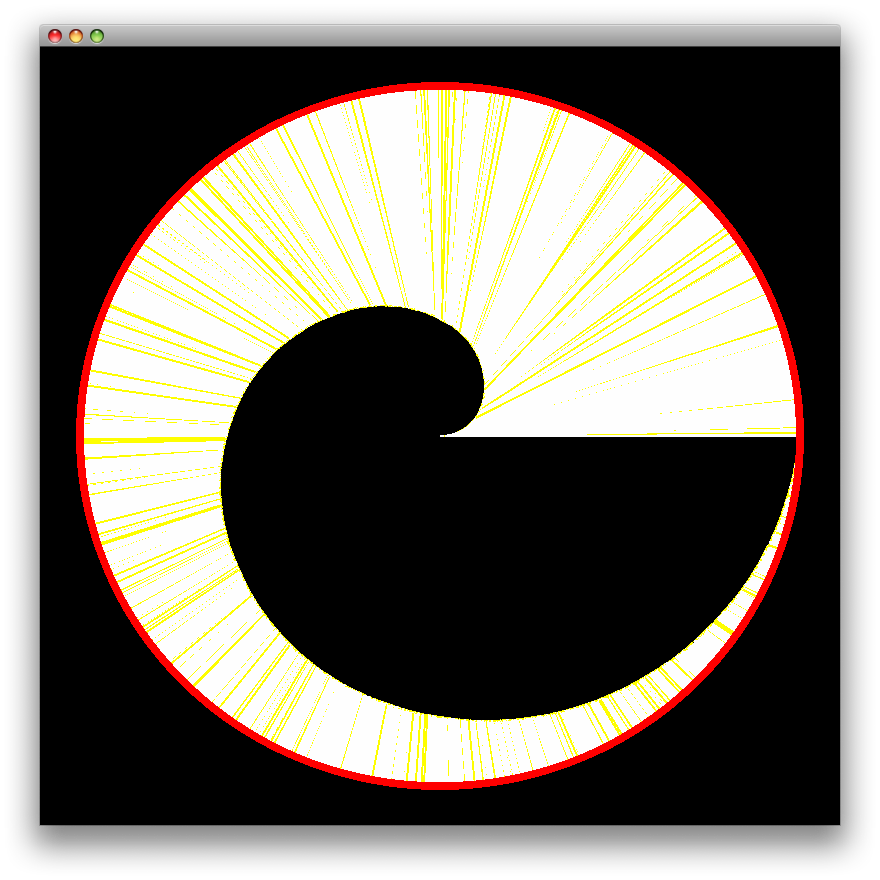
\includegraphics[scale=0.2]{pictures/cluster_jogl_impl_with_subgraph_2.png}
    \label{fig:cluster_jogl_impl_with_subgraph_2}
}
\caption{Cluster graph visualisation using improved JUNG polar dendrogram layout}
\end{figure}

As was showed before in the Figure~\ref{fig:Cytoscape_Cluster_2} cluster graph structure is specific it is very high and unbalanced with not so deep sub-parts. It is possible to use this disadvantage as advantage and abstract sub-parts to reduce drawing area. Extract those nodes and edges that form the longest path of the cluster graph - ,,backbone''. Backbone vertices are filled with yellow and showed on the Figure~\ref{fig:cluster_visualisation}. Next step is to abstract branches as a for our Spiral Tree Layout implementation. We represent this backbone as a spiral, thus preserving space and giving us a possibility to show the complete tree in one view The sub-parts are drawn as rectangles, the rectangle size represents amount of vertices inside. Figure~\ref{fig:cluster_visualisation_algorithm} shows how this approach works.

\begin{figure}[h!]
\centering
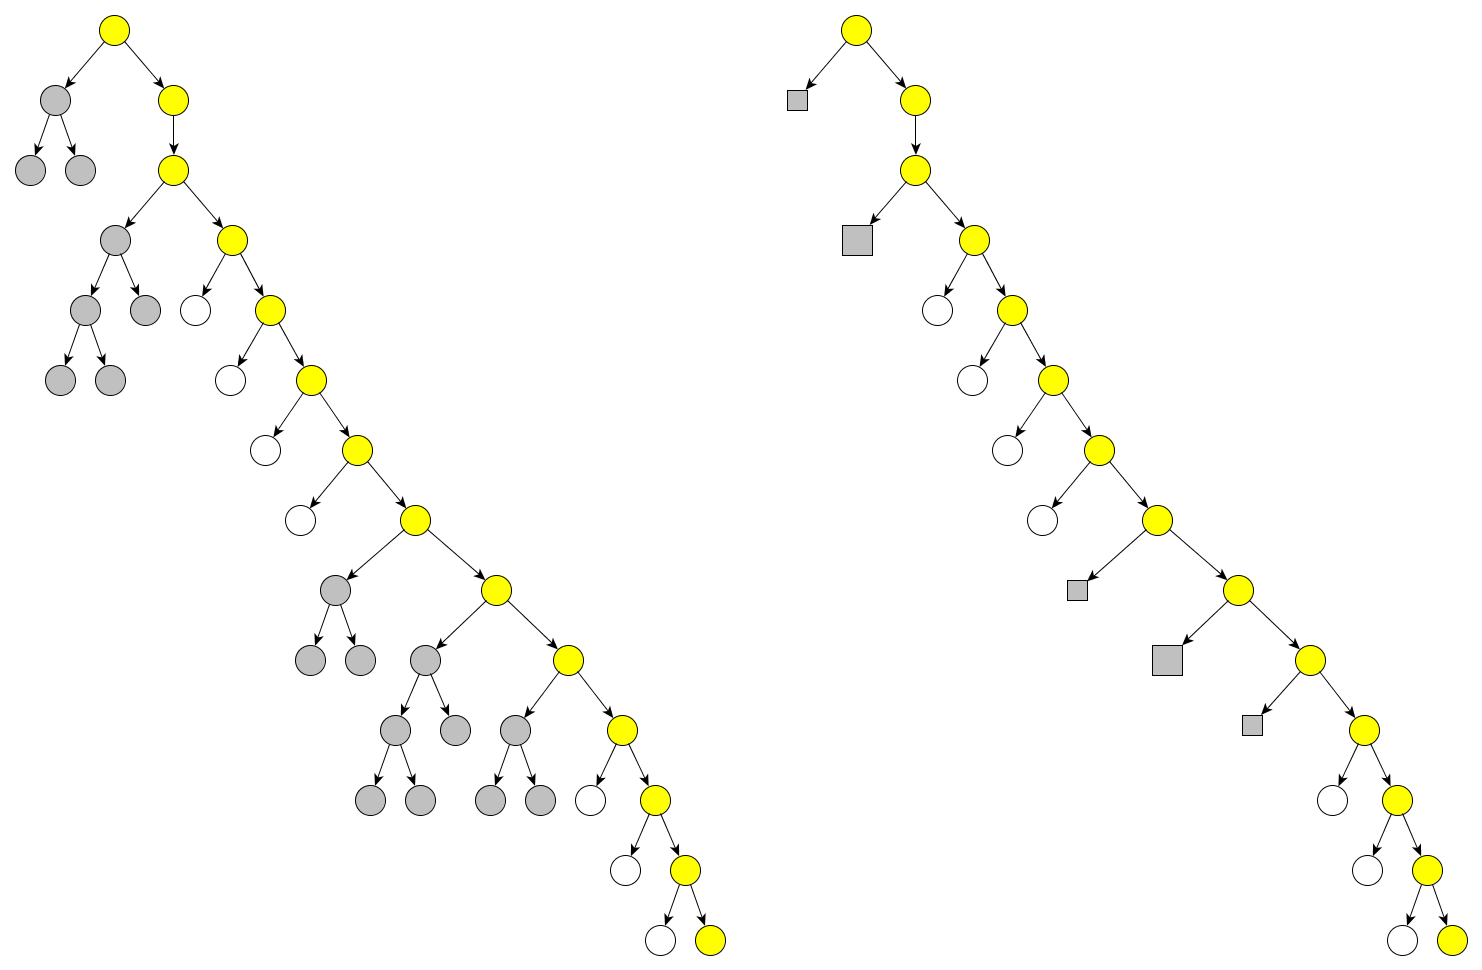
\includegraphics[scale=0.25]{pictures/cluster_visualisation_algorithm.png}
\caption{Cluster graph sub-parts abstraction}
\label{fig:cluster_visualisation_algorithm}
\end{figure}

Then backbone formed as rectangular spiral with a root in the center and moving in clockwise direction. Figure~\ref{fig:cluster_visualisation} shows complete visualisation result. This will have to reuse space as much as possible and still gives overview of location of the highlighted vertices in cluster hierarchy -- how far from a root.

\begin{figure}[h!]
\centering
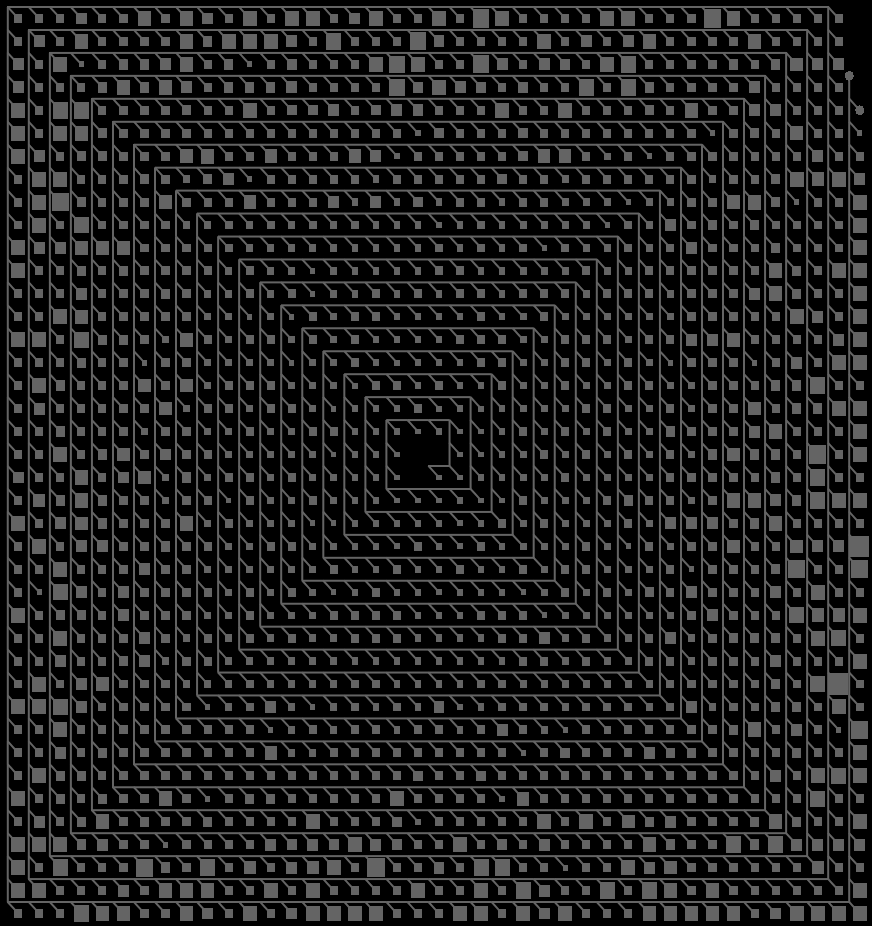
\includegraphics[scale=0.4]{pictures/cluster_visualisation.png}
\caption{Rectangular spiral Cluster graph visualisation}
\label{fig:cluster_visualisation}
\end{figure}

It is possible to explore sub-part (rectangles) of the Cluster graph using lens. User can interactively choose any sub-part and lens with inned content will appear. There are two different lens layouts: polar~\ref{fig:lens_polar} and HV-tree~\ref{fig:lens_tree}. Both implementations are own made and are not depend of any external library.

\begin{figure}[h!]
\centering
\subfloat[Polar lens layout]{
    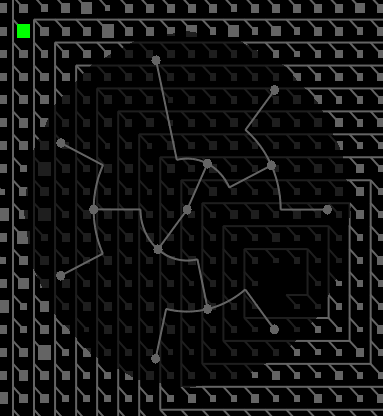
\includegraphics[scale=0.5]{pictures/lens_polar.png}
    \label{fig:lens_polar}
}
\\
\subfloat[HV-tree lens layout]{
    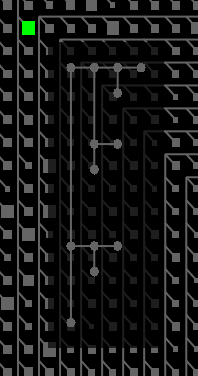
\includegraphics[scale=0.5]{pictures/lens_tree.png}
    \label{fig:lens_tree}
}
\caption{Lens layouts}
\end{figure}


\subsection{Gene Ontology Visualization}
\label{sec:go}

There are two visualisation implementations for Gene Ontology. The first layering approach is called Levels Layout and places the leaves (red pixels) and nodes (white pixels) into their corresponding layer depending on their graph-theoretic distance from the root. Moreover, leaf nodes are distributed in the left part of their assigned layer; all other nodes are arranged on the right. This feature gives us further insight into the topology of a specific layer by gaining information about the distribution of leaf nodes and non-terminal nodes on a particular layer. Figure~\ref{fig:go_levels_layout_selected} shows an example of this layout strategy in the GO view on the left hand side, whereas Figure~\ref{fig:go_zoom} displays the situation if the user zooms in the view. Although the resulting visualization looks to mimic bar charts, the number of leaves cannot be precisely compared between different layers, as the area the red node pixels (leaves) cover is not proportional to the total number of leaves in each layer. But, it is proportional to the sum of nodes in that particular layer. In other words, the covered area depends on the specific layer density. There are unconnected components in the Gene Ontology graph. Unconnected nodes are placed in the top layer number -- zero. There is an option to show-hide unconnected components from the main menu. The spatial arrangement of the node pixels within a layer, except the placing of leaves and nodes in specific regions, is random.

Second layering approach Bottom Layout is similar to the first one in terms of placing the nodes into corresponding layers based on the distance from the source node and random distribution of the node pixels within each layer. However, all leaves are placed into one single layer together with unconnected nodes at the bottom of the GO view, i. e., in the layer with the highest number. Unconnected nodes can be filtered out if necessary. This approach gives insight into the distribution of nodes among different layers without the distraction of the leaves, thus enriching the perception of the graph topology. More screenshots can be found in the Appendix~C.

\begin{figure}[h!]
\centering
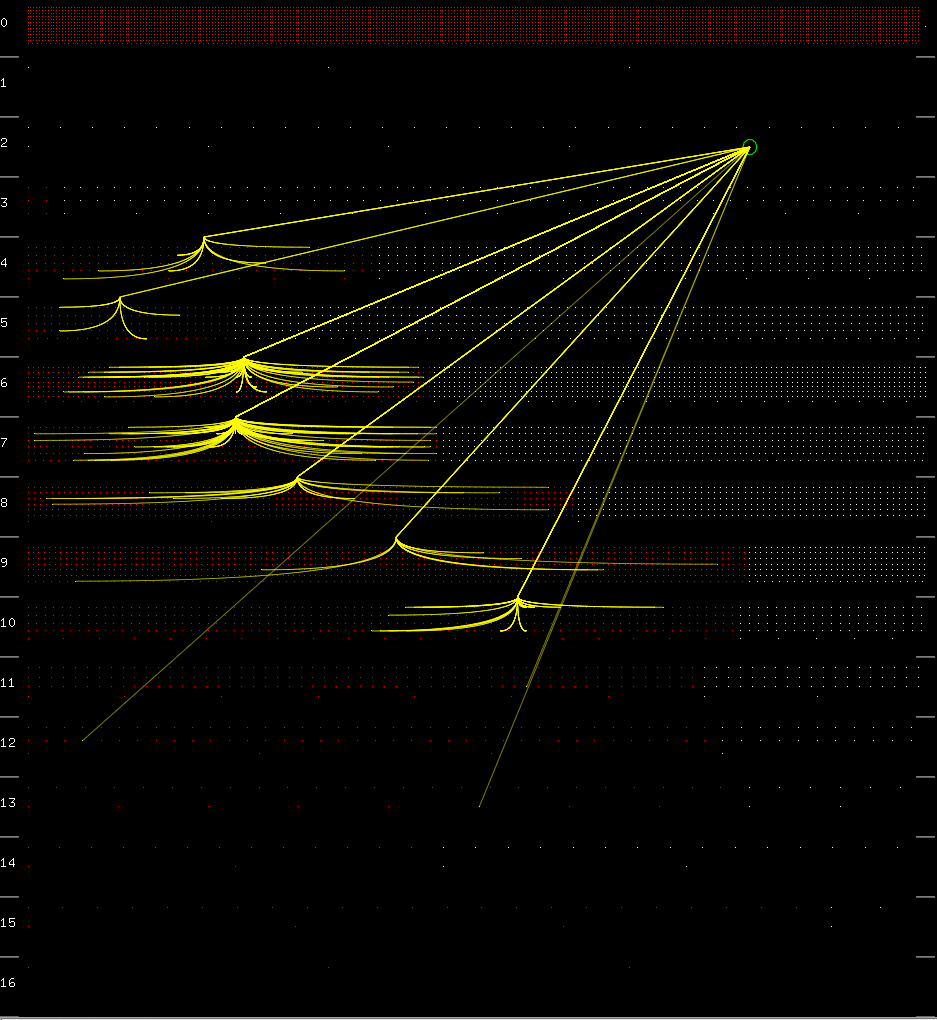
\includegraphics[scale=0.45]{pictures/go_levels_layout_selected.png}
\caption{Levels Layout visualisation with sub-graph edges}
\label{fig:go_levels_layout_selected}
\end{figure}

\begin{figure}[h!]
\centering
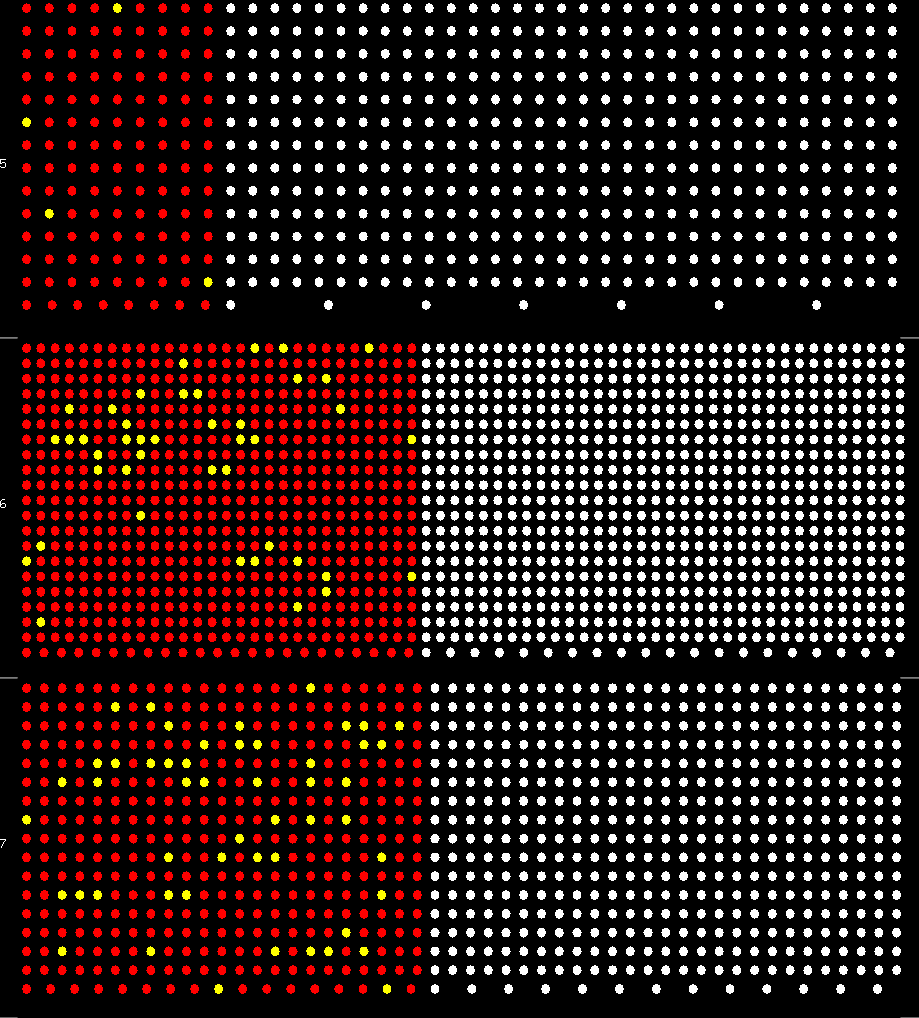
\includegraphics[scale=0.45]{pictures/go_zoom.png}
\caption{Zoomed view}
\label{fig:go_zoom}
\end{figure}

